\documentclass[5pt,aspectratio=169]{beamer}
\usetheme{metropolis}
%\usecolortheme{whale}
\usepackage{tikz}
\usetikzlibrary{decorations.pathmorphing}
\usepackage{listings}
\usepackage{amsmath}
\usepackage{xcolor}
\usepackage[normalem]{ulem} % Provides \sout for strikeout
\usetikzlibrary{arrows,shapes,positioning,fit,arrows.meta,backgrounds,calc}

% Code listing setup
\lstset{
  basicstyle=\footnotesize\ttfamily,
  breaklines=true,
  commentstyle=\color{green!60!black},
  keywordstyle=\color{blue},
  stringstyle=\color{red},
  numbers=left,
  numberstyle=\tiny\color{gray},
  backgroundcolor=\color{gray!10},
  frame=single,
  tabsize=2
}

\title{Foundations of Deep Learning \& the Emergence of Generative AI}
%\subtitle{Session 1}
\author{Mari Ganesh Kumar}
\date{\today}
%\institute{[Institution]}

\begin{document}

%% Title Slide
\begin{frame}
\titlepage
\end{frame}

%% Slide 3: Learning Objectives



\begin{frame}
\frametitle{Course Outline}
\begin{itemize}
    \item Foundations of Deep Learning \& Emergence of Generative AI
    \item VAEs
    \item GANs
    \item Auto-regressive generative models
\end{itemize}
\end{frame}

\section{About Me}

\section{About You}

\begin{frame}
    \begin{figure}
        \centering
        
\includegraphics[width=0.5\linewidth]{images/image.png}
        \label{fig:enter-label}
    \end{figure}
    \centering
     \href{https://forms.gle/C5ka9tqLZQnzY9Qx7}{click here}
\end{frame}


\begin{frame}
\frametitle{Session Learning Objectives}
By the end of this session, you will be able to:
\begin{itemize}
    \item Understand the evolution from traditional ML to deep learning
    \item Explain fundamental neural network architectures and their components
    \item Describe how deep learning innovations led to generative AI
    \item Implement a basic autoencoder for image reconstruction
\end{itemize}
\end{frame}

\begin{frame}
\frametitle{%
    \alt<1>{What is Generative AI?}{%
      \alt<2>{What is Generative \texorpdfstring{\sout{AI} Modeling}{AI}?}{%
        \texorpdfstring{What is a simple Generative \sout{AI Modeling} Model?}{Generative Modeling}}%
    }%
  }

\begin{itemize}
\item<4-> Observed Data
\[
X: H, T, H, H, T
\]
\item<5-> How can we continue generating data based on observed data?
\[
\hat{X}: H, T, H, H, T, ?, ?, ?, ?
\]
\item<6-> Let's compress the data into a parameter (not using ML simple Math)
\[
\theta = \frac{\#\text{Heads}}{N} = \frac{3}{5} = 0.6
\]
\item<7-> Let's compress the data into a parameter (in ML world)
\[
\text{maximize likelihood of $\theta $  } \rightarrow \; \arg\max_{\theta}L(\theta; X) = \arg\max_{\theta}\prod_{i=1}^{n} \theta^{x_i}(1-\theta)^{1-x_i} = 0.6
\]
\end{itemize}
\end{frame}

\begin{frame}
\frametitle{%
        \texorpdfstring{What is a simple Generative \sout{AI Modeling} Model?}{Generative Modeling}%
  }

\begin{itemize}
\item<1-> Observed Data
\[
X: H, T, H, H, T
\]
\item<1-> How can we continue generating data based on observed data?
\[
\hat{X}: H, T, H, H, T, ?, ?, ?, ?
\]
\item<1-> We compressed the data into a parameter (  $\theta = 0.6 $)
\item<2-> How do we generate data using $\theta$ 
\begin{itemize}
\item<3->$\text{Generate } u \text{ as a random number between } 0  \text{ and } 1 \text{. If } u<\theta \text{, then }\hat{X}=H\text{; else, }\hat{X}=T$
\end{itemize}
\end{itemize}
\end{frame}

% \begin{frame}{What is Generative Modelling?}
% \begin{itemize}
%     \item H,T,T,H,H,.. ->[]-> $\theta$ ->[] ->   Generated data
%     \item Image-1, Image-2, Image-3 ->[Model Training]-> $\theta$ -> [Inference] ->   Generated data
%     \item Text, Text, Text ->[Model Training]-> $\theta$ -> [Inference] ->   Generated data
    
% \end{itemize}
    
% \end{frame}



\begin{frame}{What is Generative Modelling?}
\begin{itemize}
    \item \textbf{Coin Flips}
    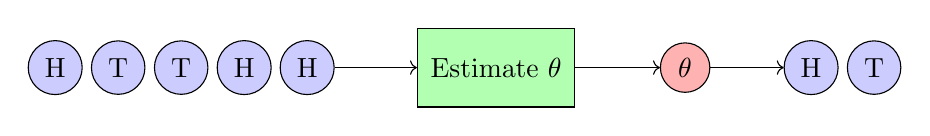
\begin{tikzpicture}[scale=0.8]
        % Original data
        \node[draw,circle,fill=blue!20] (h1) at (0,0) {H};
        \node[draw,circle,fill=blue!20] (t1) at (1,0) {T};
        \node[draw,circle,fill=blue!20] (t2) at (2,0) {T};
        \node[draw,circle,fill=blue!20] (h2) at (3,0) {H};
        \node[draw,circle,fill=blue!20] (h3) at (4,0) {H};
        
        % Model training
        \node[draw,rectangle,fill=green!30,minimum width=2cm,minimum height=1cm] (model) at (7,0) {Estimate $\theta$};
        \node[draw,circle,fill=red!30] (theta) at (10, 0) {$\theta$};
        
        % Generated data
        \node[draw,circle,fill=blue!20] (gh1) at (12,0) {H};
        \node[draw,circle,fill=blue!20] (gt1) at (13,0) {T};
        
        % Arrows
        \draw[->] (h3) -- (model);
        \draw[->] (model) -- (theta);
        \draw[->] (theta) -- (gh1);
        %\draw[->] (theta) -- (gt1);
    \end{tikzpicture}
    
    \item \textbf{Image Generation Example:}
    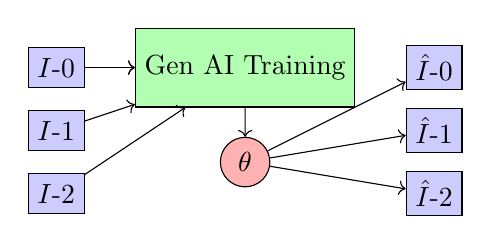
\begin{tikzpicture}[scale=0.8]
        % Original images
        \foreach \i in {0,1,2} {
            \node[draw,rectangle,fill=blue!20,minimum size=0.5cm] (I\i) at (0,-\i) {$I$-\i};
        }
        
        % Model training
        \node[draw,rectangle,fill=green!30,minimum width=2cm,minimum height=1cm] (model) at (3,0) {Gen AI Training};
        \node[draw,circle,fill=red!30] (theta) at (3,-1.5) {$\theta$};
        
        % Generated image
        \foreach \i in {0,1,2} {
            \node[draw,rectangle,fill=blue!20,minimum size=0.5cm] (i\i) at (6,-\i) {$\hat{I}$-\i};
        }

        
        % Arrows
        \foreach \i in {0,1,2} {
            \draw[->] (I\i) -- (model);
            \draw[->] (theta) -- (i\i);
        }
        \draw[->] (I0) -- (model);
        \draw[->] (model) -- (theta);
    \end{tikzpicture}
    
    \item \textbf{Text Generation Example:}
    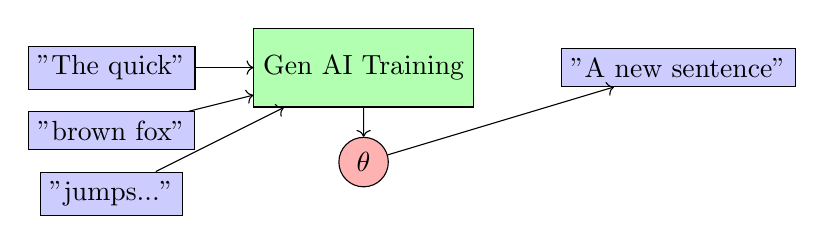
\begin{tikzpicture}[scale=0.8]
        % Original text
        \node[draw,rectangle,fill=blue!20] (text1) at (0,0) {"The quick"};
        \node[draw,rectangle,fill=blue!20] (text2) at (0,-1) {"brown fox"};
        \node[draw,rectangle,fill=blue!20] (text3) at (0,-2) {"jumps..."};
        
        % Model training
        \node[draw,rectangle,fill=green!30,minimum width=2cm,minimum height=1cm] (model) at (4,0) {Gen AI Training};
        \node[draw,circle,fill=red!30] (theta) at (4,-1.5) {$\theta$};
        
        % Generated text
        \node[draw,rectangle,fill=blue!20] (gtext) at (9,0) {"A new sentence"};
        
        % Arrows
         \foreach \i in {1,2,3} {
            \draw[->] (text\i) -- (model);
        }
        \draw[->] (model) -- (theta);
        \draw[->] (theta) -- (gtext);
    \end{tikzpicture}
\end{itemize}
\end{frame}

\begin{frame}{What is Generative AI?}

\begin{center}
\large{Common Pattern: Data $\rightarrow$ Learn Parameters $\rightarrow$ Generate New Samples}
\end{center}
\only<2->{
Today's GEN AI models can learn and generate any data (to a decent accuracy)
\begin{itemize}
    \item<3-> Generate Code, Code which solves a given task, Generate testcases given code 
    \item<4-> Generate Images, Videos, Speech, Music and turn any given image into a Ghlibli style
    \item<5-> Generate movements for a robot to navigate the physical world
    \item etc,etc
\end{itemize}
}
\only<3->{These models are getting better that all the above tasks, as we speak}
    
\end{frame}


%%% Slide 1: Probability Basics %%%
\begin{frame}{Core Probability Concepts}
\begin{columns}[T]
\begin{column}{0.48\textwidth}
\textbf{Key Definitions:}
\begin{itemize}
\item \textbf{Sample Space} ($\Omega$): All possible outcomes
\item \textbf{Event} ($E \subseteq \Omega$): Subset of outcomes
\item \textbf{Probability}: $P(E) \in [0,1]$ with:
\begin{itemize}
\item $P(\Omega) = 1$
\item $P(\bigcup_i E_i) = \sum_i P(E_i)$ for disjoint events
\end{itemize}
\end{itemize}
\end{column}

\begin{column}{0.48\textwidth}
\textbf{Random Variables:}
\begin{itemize}
\item Maps outcomes to numbers
\item Discrete vs Continuous
\item PMF/PDF: $p_X(x) = P(X=x)$
\end{itemize}

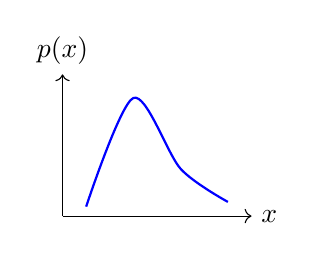
\begin{tikzpicture}[scale=0.6]
\draw[->] (0,0) -- (4,0) node[right] {$x$};
\draw[->] (0,0) -- (0,3) node[above] {$p(x)$};
\draw[blue,thick] plot[smooth] coordinates {(0.5,0.2) (1.5,2.5) (2.5,1) (3.5,0.3)};
\end{tikzpicture}
\end{column}
\end{columns}

\vspace{0.5cm}
\textbf{GenAI Connection:} All generative models learn probability distributions $p(x)$ over data space
\end{frame}

%%% Slide 2: Key Distributions %%%
\begin{frame}{Essential Probability Distributions}
\begin{columns}[T]
\begin{column}{0.33\textwidth}
\textbf{Bernoulli:}
\[ P(X=k) = \begin{cases}
p & k=1 \\
1-p & k=0
\end{cases} \]
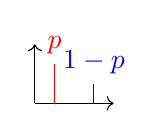
\begin{tikzpicture}[scale=0.5]
\draw[->] (0,0) -- (2,0);
\draw[->] (0,0) -- (0,1.5);
\draw[red] (0.5,0) -- (0.5,1) node[above] {$p$};
\draw[blue] (1.5,0) -- (1.5,0.5) node[above] {$1-p$};
\end{tikzpicture}
\end{column}

\begin{column}{0.33\textwidth}
\textbf{Categorical:}
\[ P(X=k) = p_k \]
\[ \text{where } \sum p_k = 1 \]
\begin{tikzpicture}[scale=0.5]
\foreach \x/\h in {0.5/1.5,1.5/1,2.5/0.8} {
    \draw[blue] (\x,0) -- (\x,\h);
}
\end{tikzpicture}
\end{column}

\begin{column}{0.33\textwidth}
\textbf{Gaussian:}
\[ p(x) = \frac{1}{\sigma\sqrt{2\pi}}e^{-\frac{(x-\mu)^2}{2\sigma^2}} \]
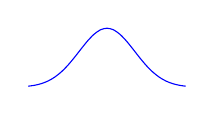
\begin{tikzpicture}[scale=0.5]
\draw[domain=-2:2,smooth,variable=\x,blue] plot ({\x+1.5},{1.5*exp(-\x*\x)});
\end{tikzpicture}
\end{column}
\end{columns}

\vspace{0.5cm}
\textbf{GenAI Usage:} Bernoulli/Categorical for discrete data, Gaussian for continuous latent spaces
\end{frame}

%%% Slide 3: Conditional Probability & Bayes %%%
\begin{frame}{Conditional Probability \& Bayes' Rule}
\begin{columns}[T]
\begin{column}{0.6\textwidth}
\textbf{Conditional Probability:}
\[ P(A|B) = \frac{P(A \cap B)}{P(B)} \]

\textbf{Bayes' Theorem:}
\[ P(A|B) = \frac{P(B|A)P(A)}{P(B)} \]

\textbf{Chain Rule:}
\[ P(X_1,\ldots,X_n) = \prod_{i=1}^n P(X_i|X_1,\ldots,X_{i-1}) \]
\end{column}

\begin{column}{0.4\textwidth}
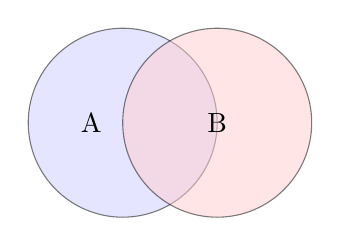
\begin{tikzpicture}[scale=0.8]
\draw[fill=blue!20, opacity=0.5] (0,0) circle (1.5);
\draw[fill=red!20, opacity=0.5] (1.5,0) circle (1.5);
\node at (-0.5,0) {A};
\node at (1.5,0) {B};
\end{tikzpicture}
\vspace{0.5cm}
\newline
\textbf{GenAI Application:} Foundation of latent variable models like VAEs:
\[ p(x|z) = \frac{p(z|x)p(x)}{p(z)} \]
\end{column}
\end{columns}


\end{frame}

%%% Slide 4: Maximum Likelihood Estimation %%%
\begin{frame}{Maximum Likelihood Estimation (MLE)}
\begin{columns}[T]
\begin{column}{0.6\textwidth}
\textbf{Objective:}
\[ \theta^* = \arg\max_\theta \prod_{i=1}^N p(x_i|\theta) \]

\textbf{Log-Likelihood:}
\[ \mathcal{L}(\theta) = \sum_{i=1}^N \log p(x_i|\theta) \]

\textbf{Example (Coin Toss):}
\[ \hat{p} = \frac{\text{\# Heads}}{N} \]
\end{column}

\begin{column}{0.4\textwidth}
\begin{tikzpicture}[scale=0.7]
\draw[->] (-1.5,0) -- (1.5,0);
\foreach \x in {-1,0,1} {
    \draw (\x,0) -- (\x,-0.1) node[below] {$\x$};
}
\draw[blue,thick] (0.6,0) -- (0.6,1.5);
\node[blue] at (0.6,1.8) {$\hat{p}$};
\end{tikzpicture}

\vspace{0.5cm}
\textbf{GenAI Connection:} Foundation for training most generative models:
\begin{itemize}
\item Explicit models: Directly maximize likelihood
\item Implicit models: Adversarial training objectives
\end{itemize}
\end{column}
\end{columns}
\end{frame}





%%% Slide 8: From Probability to GenAI %%%
\begin{frame}{Connecting Probability to Generative AI}
\begin{center}
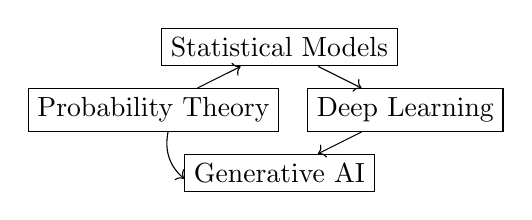
\begin{tikzpicture}[scale=0.8]
\node[draw] (prob) at (0,0) {Probability Theory};
\node[draw] (stats) at (2,1) {Statistical Models};
\node[draw] (dl) at (4,0) {Deep Learning};
\node[draw] (genai) at (2,-1) {Generative AI};

\draw[->] (prob) -- (stats);
\draw[->] (stats) -- (dl);
\draw[->] (dl) -- (genai);
\draw[->] (prob) edge[bend right] (genai);
\end{tikzpicture}
\end{center}

\textbf{Key Connections:}
\begin{itemize}
\item Neural networks $\rightarrow$ flexible function approximators
\item Gradient-based optimization of probabilistic objectives
\item Scalable inference $\rightarrow$ stochastic sampling methods
\end{itemize}
\end{frame}

%% Slide 6: Traditional ML vs Deep Learning
\begin{frame}
\frametitle{From Traditional ML to Deep Learning}
\begin{columns}
\begin{column}{0.48\textwidth}
\textbf{Traditional Machine Learning:}
\begin{itemize}
    \item Relies on hand-crafted features
    \item Limited ability to process raw data
    \item Requires extensive feature engineering
    \item Often plateaus with more data
\end{itemize}
\end{column}
\begin{column}{0.48\textwidth}
\textbf{Deep Learning:}
\begin{itemize}
    \item Automatic feature extraction
    \item Works directly with raw data
    \item Features learned hierarchically
    \item Scales with data and compute
\end{itemize}
\end{column}
\end{columns}
\end{frame}

\section{History of Deep Learning}

%% Slide 7: History of Deep Learning
\begin{frame}
\frametitle{Brief History of Deep Learning}
\begin{itemize}
    \item 1940s-50s: McCulloch, Pitts, and Rosenblatt develop perceptron
    \item 1980s: Backpropagation algorithm formalized
    \item 1990s: LeCun develops LeNet for digit recognition
    \item 2006: Hinton introduces deep belief networks
    \item 2012: AlexNet wins ImageNet competition
    \item 2014-present: Explosion of deep learning research and applications
\end{itemize}
\end{frame}

%%% 1940s-1950s: Perceptron Foundations %%%
\begin{frame}
\frametitle{1940s-1950s: Birth of Artificial Neurons}

\begin{columns}[T]
\begin{column}{0.5\textwidth}
\textbf{Key Developments:}
\begin{itemize}
\item \textbf{1943:} McCulloch-Pitts Neuron
\begin{itemize}
\item First mathematical model of biological neurons
\item Binary threshold function: 
\( f(x) = \begin{cases} 
1 & \text{if } \sum w_i x_i \geq \theta \\
0 & \text{otherwise}
\end{cases} \)
\end{itemize}

\item \textbf{1958:} Rosenblatt's Perceptron
\begin{itemize}
\item First learning algorithm for neural networks
\item \textbf{Limitations:}
\begin{itemize}
\item Could only learn linearly separable patterns
\end{itemize} 

\end{itemize}
\end{itemize}
\end{column}

\begin{column}{0.5\textwidth}
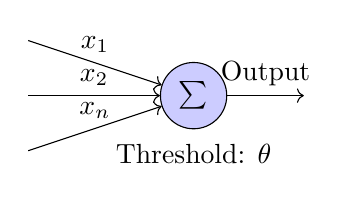
\begin{tikzpicture}[scale=0.7]
\node[draw,circle,fill=blue!20] (neuron) at (1,0) {$\sum$};
\draw[->] (-2,1) -- (neuron) node[midway,above] {$x_1$};
\draw[->] (-2,0) -- (neuron) node[midway,above] {$x_2$};
\draw[->] (-2,-1) -- (neuron) node[midway,above] {$x_n$};
\draw[->] (neuron) -- (3,0) node[midway,above] {Output};
\node[below=0.5cm] at (neuron) {Threshold: $\theta$};
\end{tikzpicture}

\vspace{0.5cm}
\textbf{Learning Rule:}
\begin{itemize}
    \item 
  \[
  w_i \leftarrow w_i + \eta(y - \hat{y})x_i
  \]
  \small{where \(\eta\) = learning rate, \(y\) = target, \(\hat{y}\) = prediction}
\item Iterative weight updates until convergence
\item Guaranteed to converge for linearly separable data
\end{itemize}

\end{column}
\end{columns}
\end{frame}



%%% Slide 1: Linear Classification Example %%%
\begin{frame}
\frametitle{Perceptron: Linear Classification Example}

\begin{columns}[T]
\begin{column}{0.5\textwidth}
\textbf{AND Gate Problem:}
\begin{itemize}
\item Inputs: \(x_1, x_2 \in \{0,1\}\)
\item Target: \(y = x_1 \land x_2\)
\end{itemize}

\textbf{Learning Process:}
\begin{enumerate}
\item Initialize weights: \(w_1=0.2, w_2=0.5, \theta=0.7\)
\item For each training example:
\begin{itemize}
\item Compute output: 
\(\hat{y} = \begin{cases} 
1 & \text{if } w_1x_1 + w_2x_2 \geq \theta \\
0 & \text{otherwise}
\end{cases}\)
\item Update weights: 
\(\Delta w_i = \eta(y - \hat{y})x_i\)
\end{itemize}
\end{enumerate}
\end{column}

\begin{column}{0.5\textwidth}
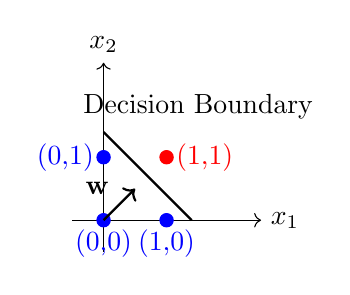
\begin{tikzpicture}[scale=0.8]
% Decision boundary: 0.5x + 0.5y = 0.7 => y = 1.4 - x
\draw[->] (-0.5,0) -- (2.5,0) node[right] {$x_1$};
\draw[->] (0,-0.5) -- (0,2.5) node[above] {$x_2$};
\draw[thick] (0.7/0.5,0) -- (0,0.7/0.5);
\node at (1.5,1.8) {Decision Boundary};

% AND gate points
\filldraw[blue] (0,0) circle (3pt) node[below] {(0,0)};
\filldraw[blue] (0,1) circle (3pt) node[left] {(0,1)};
\filldraw[blue] (1,0) circle (3pt) node[below] {(1,0)};
\filldraw[red] (1,1) circle (3pt) node[right] {(1,1)};

% Weight vector
\draw[->,thick] (0,0) -- (0.5,0.5) node[midway,above left] {\(\mathbf{w}\)};
\end{tikzpicture}

\begin{itemize}
\item Perfect linear separation
\item Achieves 100\% accuracy
\end{itemize}
\textbf{Final Learned Weights:}
\[ w_1 = 0.5, w_2 = 0.5, \theta = 0.7 \]
\end{column}
\end{columns}
\end{frame}


%%% Slide 2: Nonlinear Limitation %%%
\begin{frame}
\frametitle{Perceptron Limitation: Nonlinear Problems}

\begin{columns}[T]
\begin{column}{0.5\textwidth}
\textbf{XOR Problem:}
\begin{itemize}
\item Inputs: \(x_1, x_2 \in \{0,1\}\)
\item Target: \(y = x_1 \oplus x_2\)
\end{itemize}

\textbf{Geometric Analysis:}
\begin{itemize}
\item No single line can separate classes
\item Requires nonlinear decision boundary
\end{itemize}

\textbf{Mathematical Proof:}
\begin{align*}
0\cdot w_1 + 0\cdot w_2 &< \theta \quad (0) \\
1\cdot w_1 + 0\cdot w_2 &< \theta \quad (1) \\
0\cdot w_1 + 1\cdot w_2 &< \theta \quad (1) \\
1\cdot w_1 + 1\cdot w_2 &\geq \theta \quad (0)
\end{align*}
Contradiction: \(w_1 + w_2 \geq \theta\) but \(w_1 < \theta\), \(w_2 < \theta\)
\end{column}

\begin{column}{0.5\textwidth}
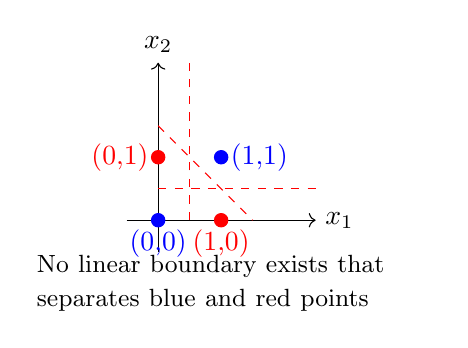
\begin{tikzpicture}[scale=0.8]
\draw[->] (-0.5,0) -- (2.5,0) node[right] {$x_1$};
\draw[->] (0,-0.5) -- (0,2.5) node[above] {$x_2$};

% XOR points
\filldraw[blue] (0,0) circle (3pt) node[below] {(0,0)};
\filldraw[red] (0,1) circle (3pt) node[left] {(0,1)};
\filldraw[red] (1,0) circle (3pt) node[below] {(1,0)};
\filldraw[blue] (1,1) circle (3pt) node[right] {(1,1)};

% Failed attempts
\draw[dashed,red] (0.5,0) -- (0.5,2.5);
\draw[dashed,red] (0,0.5) -- (2.5,0.5);
\draw[dashed,red] (0,1.5) -- (1.5,0);

\node[text width=5cm] at (1.2,-1) {
    \small{No linear boundary exists that separates blue and red points}
};
\end{tikzpicture}

\textbf{Historical Impact:}
\begin{itemize}
\item Minsky \& Papert (1969): \textit{Perceptrons} book
\item Led to first AI winter
\end{itemize}
\end{column}
\end{columns}
\end{frame}

\begin{frame}
\frametitle{Solving XOR with Logic Gates}

\textbf{Gate Combination:}
\begin{itemize}
\item OR Gate: $A + B$
\item NAND Gate: $\overline{A \cdot B}$ 
\item AND Gate: Combines previous outputs
\end{itemize}

\textbf{Boolean Expression:}
\[
XOR(A,B) = (A + B) \cdot \overline{A \cdot B}
\]
\[
= A\overline{B} + \overline{A}B
\]

\textbf{Circuit Analysis:}
\begin{enumerate}
\item OR gate detects any input activation
\item NAND gate detects non-simultaneous activation
\item AND gate ensures mutual exclusivity
\end{enumerate}

\end{frame}

\begin{frame}{How did we solve XOR using perceptron?}


\textbf{What we did right?}
\begin{itemize}
    \item<1-> Instead of single perceptron, we used multiple layers of perceptron (OR and NAND in layer 1 and AND in layer 2)
    \item<2-> We used non-linear (step function) transformation between layers
    \[
    \hat{y} = \begin{cases} 
    1 & \text{if } w_1x_1 + w_2x_2 \geq \theta \\
    0 & \text{otherwise}
    \end{cases}
    \]
    \item<3-> Most major milestones in Deep learning are because of
        \begin{itemize}
            \item increase the compute (mostly powered by hardware, trillion parameters -> today)
            \item Novel non-linearity between layers    
        \end{itemize}

\end{itemize}

\textbf{Where should we next?}
\begin{itemize}
    \item<3-> We used our domain knowledge in digital logic to design a perceptron for XOR
    \item<4-> We need to learn all the weights/parameters from data
\end{itemize}
    
\end{frame}




%%% 1980s: Backpropagation Breakthrough %%%
\begin{frame}
\frametitle{1980s: Backpropagation Revolution}

\textbf{Key Innovation:}
\begin{itemize}
\item \textbf{1986:} Rumelhart, Hinton \& Williams formalize backpropagation:
\begin{align*}
\delta^{(L)} &= (y - \hat{y}) \odot f'(z^{(L)}) \quad \text{(Output layer)} \\
\delta^{(l)} &= (W^{(l+1)T}\delta^{(l+1)}) \odot f'(z^{(l)}) \quad \text{(Hidden layers)}
\end{align*}
\end{itemize}

\begin{columns}[T]
\begin{column}{0.5\textwidth}
\textbf{Impact:}
\begin{itemize}
\item Enabled training of multi-layer networks`
\end{itemize}
\end{column}

\begin{column}{0.5\textwidth}
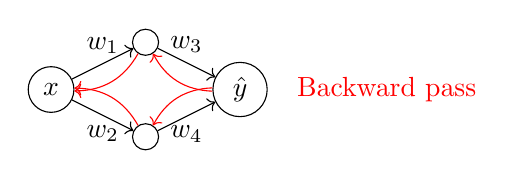
\begin{tikzpicture}[scale=0.6]
\node[draw,circle] (x) at (0,0) {$x$};
\node[draw,circle] (h1) at (2,1) {};
\node[draw,circle] (h2) at (2,-1) {};
\node[draw,circle] (y) at (4,0) {$\hat{y}$};

\draw[->] (x) -- (h1) node[midway,above] {$w_1$};
\draw[->] (x) -- (h2) node[midway,below] {$w_2$};
\draw[->] (h1) -- (y) node[midway,above] {$w_3$};
\draw[->] (h2) -- (y) node[midway,below] {$w_4$};

\draw[red,->] (y) edge[bend left] (h1);
\draw[red,->] (y) edge[bend right] (h2);
\draw[red,->] (h1) edge[bend left] (x);
\draw[red,->] (h2) edge[bend right] (x);
\node[red,right] at (5,0) {Backward pass};
\end{tikzpicture}
\end{column}
\end{columns}
\end{frame}

\begin{frame}
\frametitle{Backpropagation for XOR: Step-by-Step}

\begin{columns}[T]
\begin{column}{0.6\textwidth}
\textbf{Network Architecture:}
\begin{itemize}
\item Inputs: $x_1, x_2$ (XOR inputs)
\item Hidden Layer: 2 neurons (OR/NAND equivalents)
\item Output: 1 neuron (AND combination)
\item Activation: Sigmoid $\sigma(z) = \frac{1}{1+e^{-z}}$
\end{itemize}

\end{column}

\begin{column}{0.4\textwidth}
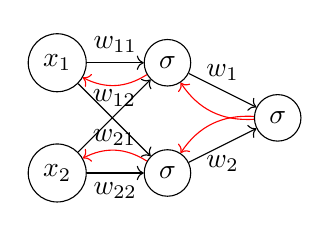
\begin{tikzpicture}[scale=0.7]
\node[draw,circle] (x1) at (0,0) {$x_1$};
\node[draw,circle] (x2) at (0,-2) {$x_2$};
\node[draw,circle] (h1) at (2,0) {$\sigma$};
\node[draw,circle] (h2) at (2,-2) {$\sigma$};
\node[draw,circle] (y) at (4,-1) {$\sigma$};

\draw[->] (x1) -- (h1) node[midway,above] {$w_{11}$};
\draw[->] (x1) -- (h2) node[midway,below] {$w_{21}$};
\draw[->] (x2) -- (h1) node[midway,above] {$w_{12}$};
\draw[->] (x2) -- (h2) node[midway,below] {$w_{22}$};
\draw[->] (h1) -- (y) node[midway,above] {$w_1$};
\draw[->] (h2) -- (y) node[midway,below] {$w_2$};

% Backprop arrows
\draw[red,->] (y) edge[bend left] (h1);
\draw[red,->] (y) edge[bend right] (h2);
\draw[red,->] (h1) edge[bend left] (x1);
\draw[red,->] (h2) edge[bend right] (x2);
\end{tikzpicture}
\end{column}
\end{columns}
\end{frame}

\begin{frame}
\frametitle{Backpropagation Mechanics for XOR Network}

\begin{columns}[T]
\begin{column}{0.6\textwidth}
\textbf{Network Structure:}
\begin{itemize}
\item \textbf{Input Layer:} $x_1, x_2$
\item \textbf{Hidden Layer:} $h_1, h_2$ with sigmoid $\sigma$
\item \textbf{Output Layer:} $\hat{y}$ with sigmoid $\sigma$
\end{itemize}

\textbf{Forward Propagation:}
\begin{align*}
z_1 &= w_{11}x_1 + w_{12}x_2 + b_1 \\
h_1 &= \sigma(z_1) \\
z_2 &= w_{21}x_1 + w_{22}x_2 + b_2 \\
h_2 &= \sigma(z_2) \\
z_3 &= w_3h_1 + w_4h_2 + b_3 \\
\hat{y} &= \sigma(z_3)
\end{align*}
\end{column}

\begin{column}{0.4\textwidth}
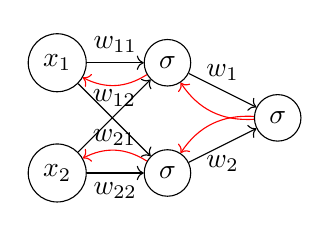
\begin{tikzpicture}[scale=0.7]
\node[draw,circle] (x1) at (0,0) {$x_1$};
\node[draw,circle] (x2) at (0,-2) {$x_2$};
\node[draw,circle] (h1) at (2,0) {$\sigma$};
\node[draw,circle] (h2) at (2,-2) {$\sigma$};
\node[draw,circle] (y) at (4,-1) {$\sigma$};

\draw[->] (x1) -- (h1) node[midway,above] {$w_{11}$};
\draw[->] (x1) -- (h2) node[midway,below] {$w_{21}$};
\draw[->] (x2) -- (h1) node[midway,above] {$w_{12}$};
\draw[->] (x2) -- (h2) node[midway,below] {$w_{22}$};
\draw[->] (h1) -- (y) node[midway,above] {$w_1$};
\draw[->] (h2) -- (y) node[midway,below] {$w_2$};

% Backprop arrows
\draw[red,->] (y) edge[bend left] (h1);
\draw[red,->] (y) edge[bend right] (h2);
\draw[red,->] (h1) edge[bend left] (x1);
\draw[red,->] (h2) edge[bend right] (x2);
\end{tikzpicture}
\end{column}
\end{columns}
\end{frame}

\begin{frame}
\frametitle{Gradient Computation Framework}

\textbf{Loss Function (MSE):}
\[
\mathcal{L} = \frac{1}{2}(y - \hat{y})^2
\]

\textbf{Chain Rule Decomposition:}
\begin{align*}
\frac{\partial \mathcal{L}}{\partial w_3} &= \underbrace{(y - \hat{y})}_{\text{Error}} \cdot \underbrace{\hat{y}(1-\hat{y})}_{\sigma'} \cdot h_1 \\
\frac{\partial \mathcal{L}}{\partial w_{11}} &= \frac{\partial \mathcal{L}}{\partial h_1} \cdot \frac{\partial h_1}{\partial z_1} \cdot x_1 
\end{align*}
\end{frame}

\begin{frame}
\frametitle{Computing Hidden Layer Gradients}

\textbf{Chain Rule Breakdown:}
\begin{align*}
\frac{\partial \mathcal{L}}{\partial w_{11}} &= 
\underbrace{\frac{\partial \mathcal{L}}{\partial \hat{y}}}_{\text{Output Error}} 
\cdot \underbrace{\frac{\partial \hat{y}}{\partial h_1}}_{\text{Weight Contribution}} 
\cdot \underbrace{\frac{\partial h_1}{\partial z_1}}_{\text{Activation Derivative}} 
\cdot \underbrace{\frac{\partial z_1}{\partial w_{11}}}_{\text{Input Value}} \\
&= (y - \hat{y}) \cdot \hat{y}(1-\hat{y}) \cdot w_3 \cdot h_1(1-h_1) \cdot x_1
\end{align*}

\textbf{Component Explanation:}
\begin{itemize}
\item $\frac{\partial \mathcal{L}}{\partial \hat{y}} = (y - \hat{y})$: Direct error measurement
\item $\frac{\partial \hat{y}}{\partial h_1} = w_3\hat{y}(1-\hat{y})$: Impact through output weight
\item $\frac{\partial h_1}{\partial z_1} = h_1(1-h_1)$: Sigmoid derivative
\item $\frac{\partial z_1}{\partial w_{11}} = x_1$: Input contribution
\end{itemize}

\end{frame}

\begin{frame}{Parallel Forward and Backward computation}
\centering
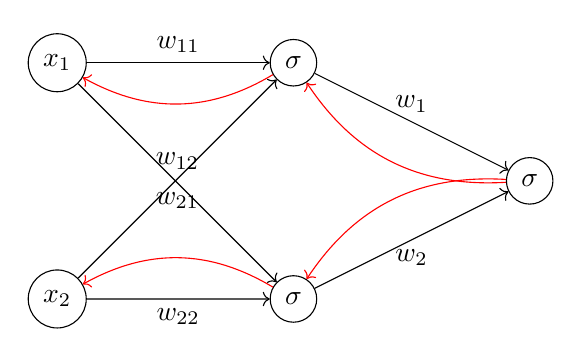
\begin{tikzpicture}[scale=1.5]
\node[draw,circle] (x1) at (0,0) {$x_1$};
\node[draw,circle] (x2) at (0,-2) {$x_2$};
\node[draw,circle] (h1) at (2,0) {$\sigma$};
\node[draw,circle] (h2) at (2,-2) {$\sigma$};
\node[draw,circle] (y) at (4,-1) {$\sigma$};

\draw[->] (x1) -- (h1) node[midway,above] {$w_{11}$};
\draw[->] (x1) -- (h2) node[midway,below] {$w_{21}$};
\draw[->] (x2) -- (h1) node[midway,above] {$w_{12}$};
\draw[->] (x2) -- (h2) node[midway,below] {$w_{22}$};
\draw[->] (h1) -- (y) node[midway,above] {$w_1$};
\draw[->] (h2) -- (y) node[midway,below] {$w_2$};

% Backprop arrows
\draw[red,->] (y) edge[bend left] (h1);
\draw[red,->] (y) edge[bend right] (h2);
\draw[red,->] (h1) edge[bend left] (x1);
\draw[red,->] (h2) edge[bend right] (x2);
\end{tikzpicture}
    
\end{frame}

\begin{frame}{Hands-On Session}
\begin{figure}
    \centering
    
\includegraphics[width=0.3\linewidth]{images/image2.png}
\end{figure}

\begin{itemize}
    \item Click here to download the file: \href{https://drive.google.com/file/d/1fNGAqAnFb2Jofu3ZP1L5prBA1-boXLli/view?usp=share_link}{Perceptron Hands-ON Session}
\end{itemize}



% gates = {
%     'or_gate': Perceptron(weights=np.array([0.5, 0.5]), threshold=0.3),
%     'nand_gate': Perceptron(weights=np.array([-0.5, -0.5]), threshold=-0.7),
%     'and_gate': Perceptron(weights=np.array([0.5, 0.5]), threshold=0.7)
%     }
    
\end{frame}

%% Slide 7: History of Deep Learning
\begin{frame}
\frametitle{Brief History of Deep Learning}
\begin{itemize}
    \item 1940s-50s: McCulloch, Pitts, and Rosenblatt develop perceptron
    \item 1980s: Backpropagation algorithm formalized
    \textbf{
    \item 1990s: LeCun develops LeNet for digit recognition
    \item 2012: AlexNet wins ImageNet competition
    }
    \item 2014-present: Explosion of deep learning research and applications
\end{itemize}
\end{frame}


%% Slide 9: What is a Neural Network?
\begin{frame}
\frametitle{What is a Neural Network?}
\begin{itemize}
    \item Computational system inspired by biological neural networks
    \item Composed of interconnected nodes (``neurons'')
    \item Learns to perform tasks by analyzing examples
    \item Excels at finding patterns in complex, high-dimensional data
    \item Universal function approximators (can theoretically learn any function)
\end{itemize}
\end{frame}

%% Slide 10: Neural Network Components
\begin{frame}
\frametitle{Neural Network Components}
\begin{itemize}
    \item \textbf{Neurons:} Computational units that process inputs
    \item \textbf{Weights:} Parameters determining input importance
    \item \textbf{Bias:} Additional parameter for flexibility
    \item \textbf{Activation Functions:} Non-linear transformations (ReLU, sigmoid, tanh)
    \item \textbf{Layers:} Collections of neurons
    \begin{itemize}
        \item Input layer
        \item Hidden layer(s)
        \item Output layer
    \end{itemize}
\end{itemize}
\end{frame}

%% Slide 11: Activation Functions
\begin{frame}
\frametitle{Common Activation Functions}
\begin{itemize}
    \item \textbf{Sigmoid:} $\sigma(x) = \frac{1}{1+e^{-x}}$
    \begin{itemize}
        \item Output range [0,1], historically common
    \end{itemize}
    \item \textbf{Tanh:} $\tanh(x) = \frac{e^x - e^{-x}}{e^x + e^{-x}}$
    \begin{itemize}
        \item Output range [-1,1], zero-centered
    \end{itemize}
    \item \textbf{ReLU:} $f(x) = \max(0,x)$
    \begin{itemize}
        \item Sparse activation, reduces vanishing gradient
    \end{itemize}
    \item \textbf{Leaky ReLU:} $f(x) = \max(\alpha x,x)$ where $\alpha$ is small
    \begin{itemize}
        \item Addresses dying ReLU problem
    \end{itemize}
    \item \textbf{Softmax:} For multi-class outputs, normalizes to probability distribution
\end{itemize}
\end{frame}

%% Slide 12: Feedforward Neural Networks
\begin{frame}
\frametitle{Feedforward Neural Networks}
\begin{columns}
\begin{column}{0.48\textwidth}
\begin{itemize}
    \item Simplest architecture, information flows in one direction
    \item Also called Multi-Layer Perceptrons (MLPs)
    \item Each neuron connected to all neurons in adjacent layers
    \item No connections between neurons in the same layer
    \item Universal function approximators
    \item Limited in handling structured data (images, sequences)
\end{itemize}
\end{column}
\begin{column}{0.48\textwidth}
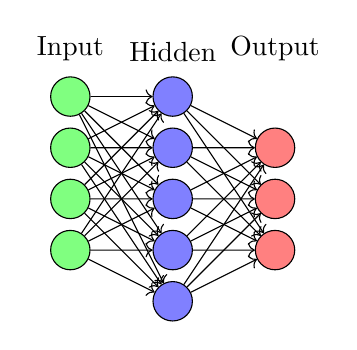
\begin{tikzpicture}[scale=0.65]
    % Define node styles
    \tikzstyle{neuron}=[circle, draw, minimum size=0.5cm]
    \tikzstyle{input neuron}=[neuron, fill=green!50]
    \tikzstyle{hidden neuron}=[neuron, fill=blue!50]
    \tikzstyle{output neuron}=[neuron, fill=red!50]
    
    % Draw input layer
    \foreach \i in {1,...,4} {
        \node[input neuron] (I-\i) at (0,-\i) {};
    }
    
    % Draw hidden layer
    \foreach \i in {1,...,5} {
        \node[hidden neuron] (H-\i) at (2,-\i) {};
    }
    
    % Draw output layer
    \foreach \i in {1,...,3} {
        \node[output neuron] (O-\i) at (4,-\i-1) {};
    }
    
    % Connect layers
    \foreach \i in {1,...,4} {
        \foreach \j in {1,...,5} {
            \draw[->] (I-\i) -- (H-\j);
        }
    }
    
    \foreach \i in {1,...,5} {
        \foreach \j in {1,...,3} {
            \draw[->] (H-\i) -- (O-\j);
        }
    }
    
    % Labels
    \node[anchor=south] at (0,-0.5) {Input};
    \node[anchor=south] at (2,-0.5) {Hidden};
    \node[anchor=south] at (4,-0.5) {Output};
\end{tikzpicture}
\end{column}
\end{columns}
\end{frame}

%% Slide 13: Convolutional Neural Networks (CNNs)
\begin{frame}
\frametitle{Convolutional Neural Networks (CNNs)}
\begin{itemize}
    \item Specialized for processing grid-like data (images)
    \item Key operations:
    \begin{itemize}
        \item \textbf{Convolution:} Filters detect local patterns
        \item \textbf{Pooling:} Reduces dimensionality, provides translation invariance
        \item \textbf{Fully connected layers:} Final classification/regression
    \end{itemize}
    \item Hierarchical feature learning:
    \begin{itemize}
        \item Early layers: Edges, textures
        \item Middle layers: Shapes, parts
        \item Deeper layers: Objects, concepts
    \end{itemize}
\end{itemize}
\end{frame}

%% Slide 14: CNN Architecture Example
\begin{frame}
\frametitle{CNN Architecture Example}
\begin{center}
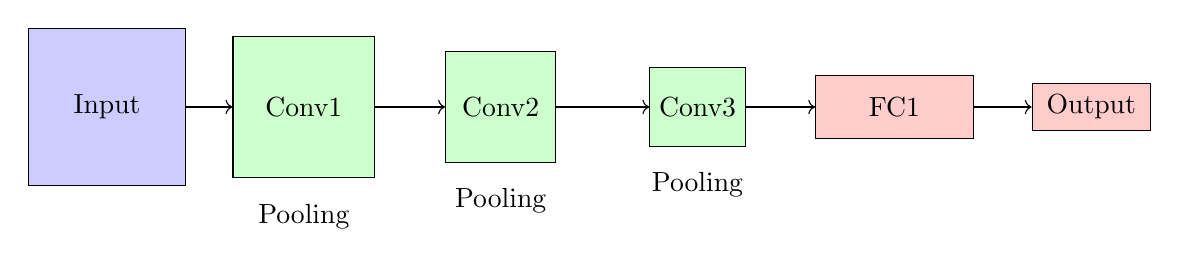
\begin{tikzpicture}[scale=0.5]
    % Input image
    \node[rectangle, minimum size=2cm, draw, fill=blue!20] (input) at (-2,0) {Input};
    
    % Convolutional layers
    \node[rectangle, minimum height=1.8cm, minimum width=1.8cm, draw, fill=green!20] (conv1) at (3,0) {Conv1};
    
    \node[rectangle, minimum height=1.4cm, minimum width=1.4cm, draw, fill=green!20] (conv2) at (8,0) {Conv2};
    
    \node[rectangle, minimum height=1cm, minimum width=1cm, draw, fill=green!20] (conv3) at (13,0) {Conv3};
    
    % Fully connected layers
    \node[rectangle, minimum height=0.8cm, minimum width=2cm, draw, fill=red!20] (fc1) at (18,0) {FC1};
    
    % Output layer
    \node[rectangle, minimum height=0.6cm, minimum width=1.5cm, draw, fill=red!20] (output) at (23,0) {Output};
    
    % Connections
    \draw[->] (input) -- (conv1);
    \draw[->] (conv1) -- (conv2);
    \draw[->] (conv2) -- (conv3);
    \draw[->] (conv3) -- (fc1);
    \draw[->] (fc1) -- (output);
    
    % Pooling operations
    \node[below=0.2cm of conv1] {Pooling};
    \node[below=0.2cm of conv2] {Pooling};
    \node[below=0.2cm of conv3] {Pooling};
\end{tikzpicture}
\end{center}

Key innovations:
\begin{itemize}
    \item Local receptive fields
    \item Parameter sharing
    \item Hierarchical feature extraction
\end{itemize}
\end{frame}


%% Slide 3: The Convolution Operation
\begin{frame}
\frametitle{Convolution Operation: The Core Mechanism}

\begin{columns}
\begin{column}{0.5\textwidth}
\textbf{Key Idea:}
\begin{itemize}
\item Slide a filter/kernel across input
\item Compute element-wise products
\item Sum products to create feature maps
\end{itemize}

\textbf{Mathematical Form:}
For 2D: 
\[ (I * K)[i,j] = \sum_{m}\sum_{n} I[i+m,j+n] \cdot K[m,n] \]

\end{column}

\begin{column}{0.5\textwidth}
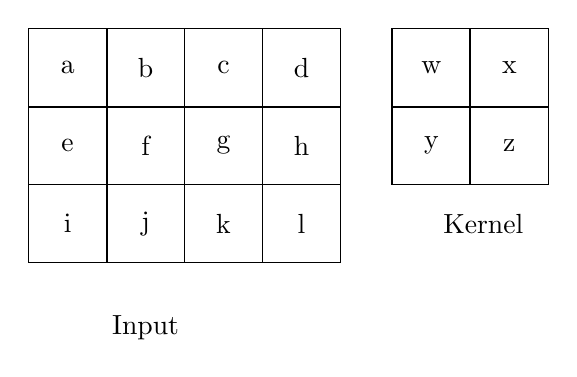
\begin{tikzpicture}[scale=0.66]
% Input grid
\node[draw, minimum size=1cm] (a) at (0,0) {a};
\node[draw, minimum size=1cm] (b) at (1.5,0) {b};
\node[draw, minimum size=1cm] (c) at (3,0) {c};
\node[draw, minimum size=1cm] (d) at (4.5,0) {d};
\node[draw, minimum size=1cm] (e) at (0,-1.5) {e};
\node[draw, minimum size=1cm] (f) at (1.5,-1.5) {f};
\node[draw, minimum size=1cm] (g) at (3,-1.5) {g};
\node[draw, minimum size=1cm] (h) at (4.5,-1.5) {h};
\node[draw, minimum size=1cm] (i) at (0,-3) {i};
\node[draw, minimum size=1cm] (j) at (1.5,-3) {j};
\node[draw, minimum size=1cm] (k) at (3,-3) {k};
\node[draw, minimum size=1cm] (l) at (4.5,-3) {l};

\node at (1.5,-5) {Input};

% Kernel
\node[draw, minimum size=1cm] (w) at (7,0) {w};
\node[draw, minimum size=1cm] (x) at (8.5,0) {x};
\node[draw, minimum size=1cm] (y) at (7,-1.5) {y};
\node[draw, minimum size=1cm] (z) at (8.5,-1.5) {z};

\node at (8,-3) {Kernel};
\end{tikzpicture}
\end{column}
\end{columns}

\end{frame}

%% Slide 4: Convolution Visualization
\begin{frame}
\frametitle{Convolution in Action}

\begin{center}
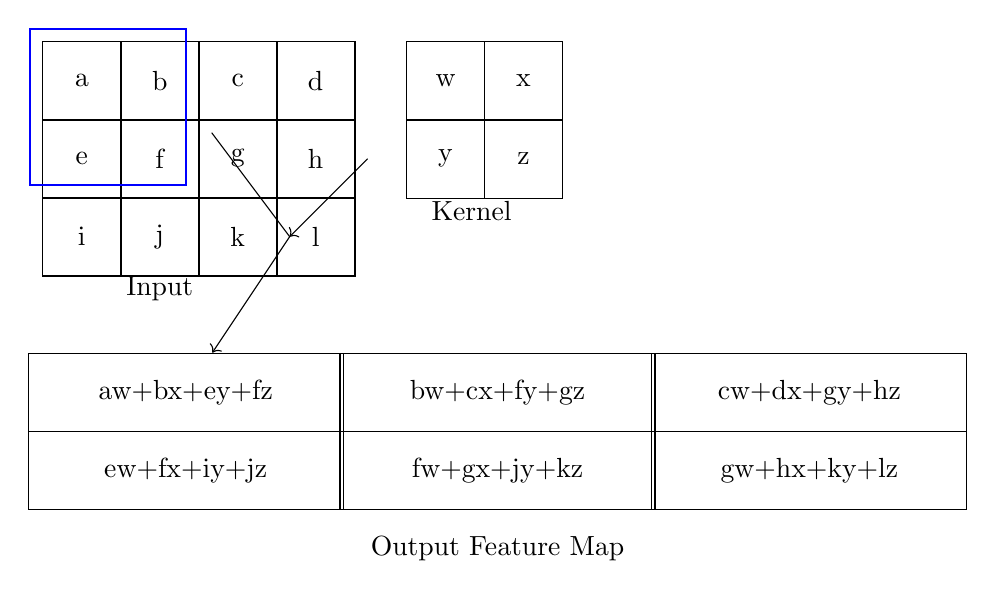
\begin{tikzpicture}[scale=0.66]
% Input grid
\node[draw, minimum size=1cm] (a) at (0,0) {a};
\node[draw, minimum size=1cm] (b) at (1.5,0) {b};
\node[draw, minimum size=1cm] (c) at (3,0) {c};
\node[draw, minimum size=1cm] (d) at (4.5,0) {d};
\node[draw, minimum size=1cm] (e) at (0,-1.5) {e};
\node[draw, minimum size=1cm] (f) at (1.5,-1.5) {f};
\node[draw, minimum size=1cm] (g) at (3,-1.5) {g};
\node[draw, minimum size=1cm] (h) at (4.5,-1.5) {h};
\node[draw, minimum size=1cm] (i) at (0,-3) {i};
\node[draw, minimum size=1cm] (j) at (1.5,-3) {j};
\node[draw, minimum size=1cm] (k) at (3,-3) {k};
\node[draw, minimum size=1cm] (l) at (4.5,-3) {l};

\node at (1.5,-4) {Input};

% Highlight first position
\draw[blue, thick] (-1,1) rectangle (2,-2);

% Kernel
\node[draw, minimum size=1cm] (w) at (7,0) {w};
\node[draw, minimum size=1cm] (x) at (8.5,0) {x};
\node[draw, minimum size=1cm] (y) at (7,-1.5) {y};
\node[draw, minimum size=1cm] (z) at (8.5,-1.5) {z};

\node at (7.5,-2.5) {Kernel};

% Output
\node[draw, minimum width=4cm, minimum height=1cm] (o1) at (2,-6) {aw+bx+ey+fz};
\node[draw, minimum width=4cm, minimum height=1cm] (o2) at (8,-6) {bw+cx+fy+gz};
\node[draw, minimum width=4cm, minimum height=1cm] (o3) at (14,-6) {cw+dx+gy+hz};
\node[draw, minimum width=4cm, minimum height=1cm] (o4) at (2,-7.5) {ew+fx+iy+jz};
\node[draw, minimum width=4cm, minimum height=1cm] (o5) at (8,-7.5) {fw+gx+jy+kz};
\node[draw, minimum width=4cm, minimum height=1cm] (o6) at (14,-7.5) {gw+hx+ky+lz};

\node at (8,-9) {Output Feature Map};

% Arrows
\draw[->] (2.5,-1) -- (4,-3) -- (o1);
\draw[->] (5.5,-1.5) -- (4,-3);
\end{tikzpicture}
\end{center}

\end{frame}


%% Slide: Transposed Convolution Visualization
\begin{frame}
\frametitle{Transposed Convolution in Action}

\begin{center}
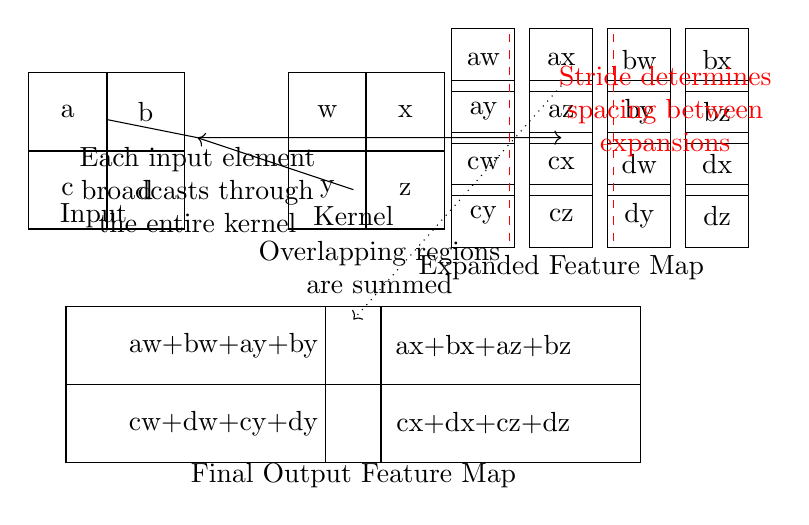
\begin{tikzpicture}[scale=0.66]
% Input grid (smaller than output)
\node[draw, minimum size=1cm] (a) at (0,0) {a};
\node[draw, minimum size=1cm] (b) at (1.5,0) {b};
\node[draw, minimum size=1cm] (c) at (0,-1.5) {c};
\node[draw, minimum size=1cm] (d) at (1.5,-1.5) {d};

\node at (0.5,-2) {Input};

% Kernel
\node[draw, minimum size=1cm] (w) at (5,0) {w};
\node[draw, minimum size=1cm] (x) at (6.5,0) {x};
\node[draw, minimum size=1cm] (y) at (5,-1.5) {y};
\node[draw, minimum size=1cm] (z) at (6.5,-1.5) {z};

\node at (5.5,-2) {Kernel};

% Output grid (larger than input)
\node[draw, minimum size=0.8cm] (o1) at (8,1) {aw};
\node[draw, minimum size=0.8cm] (o2) at (9.5,1) {ax};
\node[draw, minimum size=0.8cm] (o3) at (11,1) {bw};
\node[draw, minimum size=0.8cm] (o4) at (12.5,1) {bx};
\node[draw, minimum size=0.8cm] (o5) at (8,0) {ay};
\node[draw, minimum size=0.8cm] (o6) at (9.5,0) {az};
\node[draw, minimum size=0.8cm] (o7) at (11,0) {by};
\node[draw, minimum size=0.8cm] (o8) at (12.5,0) {bz};
\node[draw, minimum size=0.8cm] (o9) at (8,-1) {cw};
\node[draw, minimum size=0.8cm] (o10) at (9.5,-1) {cx};
\node[draw, minimum size=0.8cm] (o11) at (11,-1) {dw};
\node[draw, minimum size=0.8cm] (o12) at (12.5,-1) {dx};
\node[draw, minimum size=0.8cm] (o13) at (8,-2) {cy};
\node[draw, minimum size=0.8cm] (o14) at (9.5,-2) {cz};
\node[draw, minimum size=0.8cm] (o15) at (11,-2) {dy};
\node[draw, minimum size=0.8cm] (o16) at (12.5,-2) {dz};

\node at (9.5,-3) {Expanded Feature Map};

% Output after summation (overlapping regions)
\node[draw, minimum width=4cm, minimum height=1cm] (s1) at (3,-4.5) {aw+bw+ay+by};
\node[draw, minimum width=4cm, minimum height=1cm] (s2) at (8,-4.5) {ax+bx+az+bz};
\node[draw, minimum width=4cm, minimum height=1cm] (s3) at (3,-6) {cw+dw+cy+dy};
\node[draw, minimum width=4cm, minimum height=1cm] (s4) at (8,-6) {cx+dx+cz+dz};

\node at (5.5,-7) {Final Output Feature Map};

% Arrows and explanations
\draw[->] (a) -- (2.5,-0.5) -- (9.5,-0.5);
\draw[->] (5.5,-1.5) -- (2.5,-0.5);
\node[align=center] at (2.5,-1.5) {Each input element\\broadcasts through\\the entire kernel};

% Summation arrows
\draw[->, dotted] (9.5,0.5) -- (5.5,-4);
\node[align=center] at (6,-3) {Overlapping regions\\are summed};

% Highlight stride and expansion
\draw[red, dashed] (8.5,1.5) -- (8.5,-2.5);
\draw[red, dashed] (10.5,1.5) -- (10.5,-2.5);
\node[red, align=center] at (11.5,0) {Stride determines\\spacing between\\expansions};

\end{tikzpicture}
\end{center}

\end{frame}



%%% 1990s: LeNet Evolution %%%
\begin{frame}
\frametitle{1990s: LeNet's CNN Breakthrough}

\begin{columns}[T]
\begin{column}{0.6\textwidth}
\textbf{Architectural Innovations:}
\begin{itemize}
\item \textbf{1989:} LeNet-1 (AT\&T Bell Labs)
\begin{itemize}
\item 3 hidden layers, 9,760 parameters
\item 1\% error on USPS zip codes
\end{itemize}

\item \textbf{1998:} LeNet-5
\begin{itemize}
\item 2 Conv + 2 Pool + 3 FC layers
\item MNIST benchmark: 0.8\% error
\item First practical deployment in check reading systems
\end{itemize}
\end{itemize}

\begin{table}
\centering
\scalebox{0.7}{
\begin{tabular}{|l|c|c|c|}
\hline
\textbf{Version} & \textbf{Params} & \textbf{Error} & \textbf{Dataset} \\
\hline
LeNet-1 (1989) & 9,760 & 1\% & USPS \\
LeNet-4 (1994) & 17,000 & 0.7\% & MNIST \\
LeNet-5 (1998) & 60,000 & 0.8\% & MNIST \\
\hline
\end{tabular}
}
\end{table}
\end{column}

\begin{column}{0.4\textwidth}
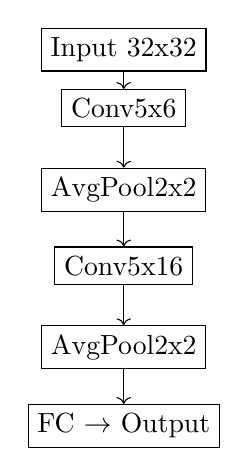
\begin{tikzpicture}[scale=0.5]
\node[draw] (input) {Input 32x32};
\node[draw,below=0.5cm] (conv1) at (0,0) {Conv5x6};
\node[draw,below=0.5cm] (pool1) at (0,-2) {AvgPool2x2};
\node[draw,below=0.5cm] (conv2) at (0,-4) {Conv5x16};
\node[draw,below=0.5cm] (pool2) at (0,-6) {AvgPool2x2};
\node[draw,below=0.5cm] (fc) at (0, -8) {FC $\rightarrow$ Output};

\draw[->] (input) -- (conv1);
\draw[->] (conv1) -- (pool1);
\draw[->] (pool1) -- (conv2);
\draw[->] (conv2) -- (pool2);
\draw[->] (pool2) -- (fc);
\end{tikzpicture}
\end{column}
\end{columns}
\end{frame}


%%% 2012: AlexNet Revolution %%%
\begin{frame}
\frametitle{2012: AlexNet's ImageNet Domination}

\begin{columns}[T]
\begin{column}{0.5\textwidth}
\textbf{ILSVRC 2012 Results:}
\begin{itemize}
\item Top-5 error: 15.3\% (vs 26.2\% second place)
\item 60M parameters, 5 Conv + 3 FC layers
\end{itemize}

\textbf{Key Innovations:}
\begin{itemize}
\item ReLU activation: \( f(x) = \max(0,x) \)
\item Dropout regularization (p=0.5)
\item Dual GPU implementation
\end{itemize}

\begin{table}
\centering
\scalebox{0.7}{
\begin{tabular}{|l|c|}
\hline
\textbf{Model} & \textbf{Top-5 Error} \\
\hline
AlexNet & 15.3\% \\
SVM & 26.2\% \\
Best 2011 Entry & 25.8\% \\
\hline
\end{tabular}
}
\end{table}
\end{column}

\begin{column}{0.5\textwidth}
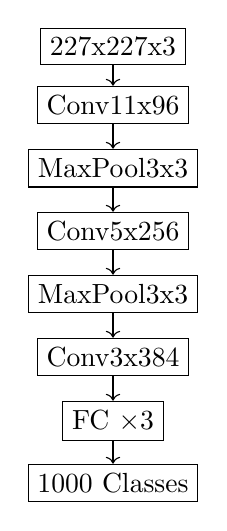
\begin{tikzpicture}[scale=0.4]
\node[draw] (input) {227x227x3};
\node[draw,below=0.5cm] (conv1) at (0,0) {Conv11x96};
\node[draw,below=0.5cm] (pool1) at (0,-2) {MaxPool3x3};
\node[draw,below=0.5cm] (conv2) at (0,-4) {Conv5x256};
\node[draw,below=0.5cm] (pool2) at (0,-6) {MaxPool3x3};
\node[draw,below=0.5cm] (conv3) at (0,-8) {Conv3x384};
\node[draw,below=0.5cm] (fc) at (0,-10) {FC $\times$3};
\node[draw,below=0.5cm] (out) at (0, -12) {1000 Classes};

\draw[->] (input) -- (conv1);
\draw[->] (conv1) -- (pool1);
\draw[->] (pool1) -- (conv2);
\draw[->] (conv2) -- (pool2);
\draw[->] (pool2) -- (conv3);
\draw[->] (conv3) -- (fc);
\draw[->] (fc) -- (out);
\end{tikzpicture}
\end{column}
\end{columns}
\end{frame}



%% Slide 8: Key Milestones in Deep Learning
\begin{frame}
\frametitle{Key Milestones in Deep Learning}
\begin{itemize}
    \item \textbf{2012:} AlexNet demonstrates power of deep CNNs \textit{(~60-62 million parameters)}
    \item \textbf{2014:} GANs introduced by Goodfellow et al.
    \item \textbf{2014:} Encoder-decoder architectures for sequence tasks \textit{(seq2seq: 384M parameters)}
    \item \textbf{2015-16:} ResNet and batch normalization \textit{(ResNet-50: ~25 million parameters)}
    \item \textbf{2017:} Transformer architecture
    \item \textbf{2018-20:} Pre-trained language models
        \begin{itemize}
            \item BERT-Base: 108.8 million parameters
            \item GPT-3: 175 billion parameters
        \end{itemize}
    \item \textbf{2021-present:} Large-scale generative models
        \begin{itemize}
            \item DALL-E: 12 billion parameters
            \item DALL-E 2: 3.5 billion parameters
            \item Stable Diffusion 3.5 Large: 8.1 billion parameters
            \item GPT-4: estimated 1.8 trillion parameters
        \end{itemize}
\end{itemize}
\end{frame}


%%% 2014-Present: Deep Learning Explosion %%%
\begin{frame}
\frametitle{2014-Present: Generative AI Revolution}

\begin{columns}[T]
\begin{column}{0.5\textwidth}
\textbf{Key Developments:}
\begin{itemize}
\item \textbf{2013:} VAEs (Variational Auto-encoding)
\item \textbf{2014:} GANs (Generative Adversarial Networks)
\item \textbf{2015:} ResNets (152 layers)
\item \textbf{2017:} Transformer Architecture (Auto-regressive Gen AI)
\item \textbf{2020:} Diffusion Models, VQ-VAE
\item \textbf{2022:} ChatGPT (175B params), RVQ
\item \textbf{2024:-} Multimodal LLMs, Agentic LLMs
\end{itemize}
\end{column}


\begin{column}{0.5\textwidth}
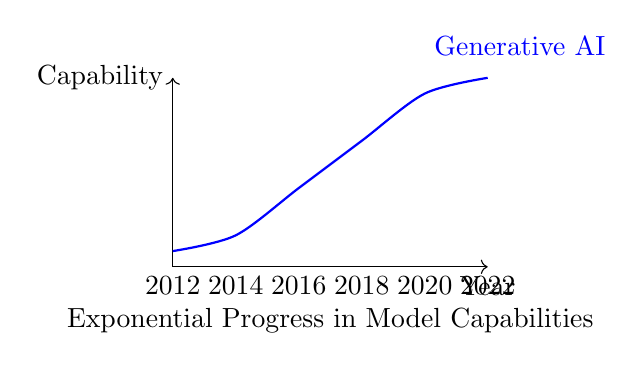
\begin{tikzpicture}[scale=0.4]
\draw[->] (0,0) -- (10,0) node[below] {Year};
\draw[->] (0,0) -- (0,6) node[left] {Capability};

\foreach \x/\y in {2012/1, 2014/2, 2016/3, 2018/4, 2020/5, 2022/6} {
    \node[below] at (\x-2012,0) {\x};
}

\draw[blue,thick] plot[smooth] coordinates {
    (0,0.5)(2,1)(4,2.5)(6,4)(8,5.5)(10,6)
};

\node[blue,right] at (8,7) {Generative\ AI};
\node[below] at (5,-1) {Exponential Progress in Model Capabilities};
\end{tikzpicture}
\textbf{Performance Growth:}
\begin{itemize}
\item Compute: 10x/year since 2012
\item Model size: 5700x increase (2012-2023)
\end{itemize}
\end{column}
\end{columns}


\end{frame}





%% Slide 18: Introduction to Generative AI
\begin{frame}
\frametitle{Introduction to Generative AI}
\begin{itemize}
    \item Models that create new content rather than classify/predict
    \item Can generate images, text, audio, video, 3D models, etc.
    \item Learn underlying data distributions
    \item Represent a fundamental shift from discriminative to creative AI
    \item Applications across art, design, content creation, science, and more
\end{itemize}
\end{frame}

%% Slide 19: Discriminative vs. Generative Models
\begin{frame}
\frametitle{Discriminative vs. Generative Models}
\begin{columns}
\begin{column}{0.48\textwidth}
\textbf{Discriminative Models:}
\begin{itemize}
    \item \textbf{Learn} decision \textbf{boundaries} between classes
    \item<2-> Model $P(Y|X)$ - probability of label given input
    \item<3-> Focus on classification/regression tasks
    \item<4-> Examples: CNN classifiers, logistic regression
\end{itemize}
\end{column}
\begin{column}{0.48\textwidth}
\textbf{Generative Models:}
\begin{itemize}
    \item \textbf{Learn} to generate data resembling training \textbf{distribution}
    \item<2-> Model $P(X)$ or $P(X,Y)$ - probability of data (and labels)
    \item<3-> Can create new instances from learned distribution
    \item<4-> Examples: GANs, VAEs, diffusion models
\end{itemize}
\end{column}
\end{columns}

\end{frame}

%% Slide 20: Examples of Discriminative & Generative Tasks
\begin{frame}
\frametitle{Examples of Discriminative \& Generative Tasks}
\begin{columns}
\begin{column}{0.48\textwidth}
\textbf{Discriminative Examples:}
\begin{itemize}
    \item \textbf{MNIST Classification:} 
    \begin{itemize}
        \item Input: Handwritten digit image
        \item Output: Probability over 10 classes
        \item Model: $P(digit|image)$
    \end{itemize}
    \item \textbf{Speaker Identification:}
    \begin{itemize}
        \item Input: Voice recording
        \item Output: Speaker identity
        \item Model: $P(speaker|audio)$
    \end{itemize}
\end{itemize}
\end{column}

\begin{column}{0.48\textwidth}
\textbf{Generative Examples:}
\begin{itemize}
    \item \textbf{Image Generation:}
    \begin{itemize}
        \item Input: Random noise/text prompt
        \item Output: Novel synthetic image 
        \item Model: $P(image)$ or $P(image|text)$
    \end{itemize}
    \item \textbf{Speech Recognition (ASR):}
    \begin{itemize}
        \item Input: Audio waveform
        \item Output: Text transcript
        \item Model: $P(text|audio)$
    \end{itemize}
\end{itemize}
\end{column}
\end{columns}

\begin{center}
\begin{tabular}{|l|c|c|}
\hline
\textbf{Domain} & \textbf{Discriminative Task} & \textbf{Generative Task} \\
\hline
Image & Object Detection & Image Synthesis \\
Speech & Speaker ID & Speech Generation \\
Text & Sentiment Analysis & Text Generation \\
\hline
\end{tabular}
\end{center}

\textbf{Key Insight:} Many tasks can be approached from either perspective!
\end{frame}

\begin{frame}
\frametitle{Generative Models: From Traditional ML to Deep Learning}

\begin{itemize}
\item \textbf{Evolution of Generative Capability:} Generative models have evolved from simple statistical models to complex neural architectures capable of creating highly realistic content.

\item \textbf{Key Evolutionary Stages:}
  \begin{itemize}
  \item \textbf{Statistical Era (1980s-2000s):} Gaussian Mixture Models, Hidden Markov Models
  \item \textbf{Energy-Based Models (2000s):} Restricted Boltzmann Machines, Deep Belief Networks
  \item \textbf{Modern Deep Generative Era (2014-present):} VAEs, GANs, Diffusion Models, Transformers
  \end{itemize}

\item \textbf{Architectural Patterns:} Most successful generative models share key principles:
  \begin{itemize}
  \item Latent space representations (compression of data distributions)
  \item Hierarchical feature learning (from pixels to concepts)
  \item Iterative refinement (progressive improvement of generations)
  \end{itemize}
\end{itemize}
\end{frame}


\begin{frame}
\frametitle{Generative Models: From Traditional ML to Deep Learning}

\begin{itemize}

\item \textbf{Convergence with Other Fields:} Recent generative AI success comes from:
  \begin{itemize}
  \item Large-scale pre-training (foundation models)
  \item Multimodal integration (text, image, audio)
  \item Human feedback and alignment techniques
  \end{itemize}
\end{itemize}
\end{frame}
%% Slide 20: Probabilistic Modeling Foundations
\begin{frame}
\frametitle{Probabilistic Modeling Foundations}
\begin{itemize}
    \item Generative models based on probability theory
    \item Core concept: modeling data distribution $P(X)$
    \item Two main approaches:
    \begin{itemize}
        \item Explicit density estimation (direct modeling)
        \item Implicit density estimation (sampling-based)
    \end{itemize}
    \item Maximum likelihood principle: find parameters that maximize probability of observed data
\end{itemize}

\begin{center}
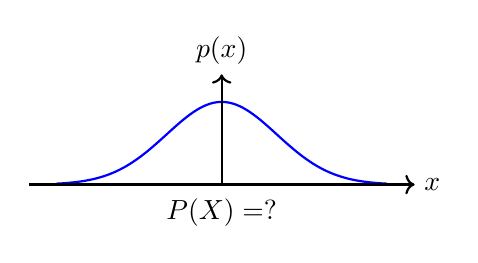
\begin{tikzpicture}[scale=0.7]
    % Draw normal distribution curve
    \draw[domain=-3:3, samples=100, smooth, variable=\x, blue, thick] 
        plot ({\x}, {1.5*exp(-(\x)^2/2)});
    
    % X-axis
    \draw[->, thick] (-3.5,0) -- (3.5,0);
    \node[right] at (3.5,0) {$x$};
    
    % Y-axis
    \draw[->, thick] (0,0) -- (0,2);
    \node[above] at (0,2) {$p(x)$};
    
    % Label
    \node at (0,-0.5) {$P(X) = ?$};
\end{tikzpicture}
\begin{figure}
    \centering
    
\includegraphics[width=0.5\linewidth]{images/image2.png}
    \caption{Enter Caption}
    \label{fig:enter-label}
\end{figure}
\end{center}
\end{frame}

%% Slide 21: Latent Representations
\begin{frame}
\frametitle{Latent Representations and Spaces}
\begin{itemize}
    \item \textbf{Latent Space:} Lower-dimensional space encoding key features
    \item High-dimensional data $\rightarrow$ compressed representation $\rightarrow$ reconstruction
    \item Properties of good latent spaces:
    \begin{itemize}
        \item Continuous
        \item Complete (covers training distribution)
        \item Disentangled (separable factors of variation)
    \end{itemize}
    \item Enable controlled generation and manipulation
\end{itemize}
\end{frame}





%% Slide 25: Evolution of Generative Capabilities
\begin{frame}
\frametitle{Evolution of Generative Capabilities}
\begin{center}
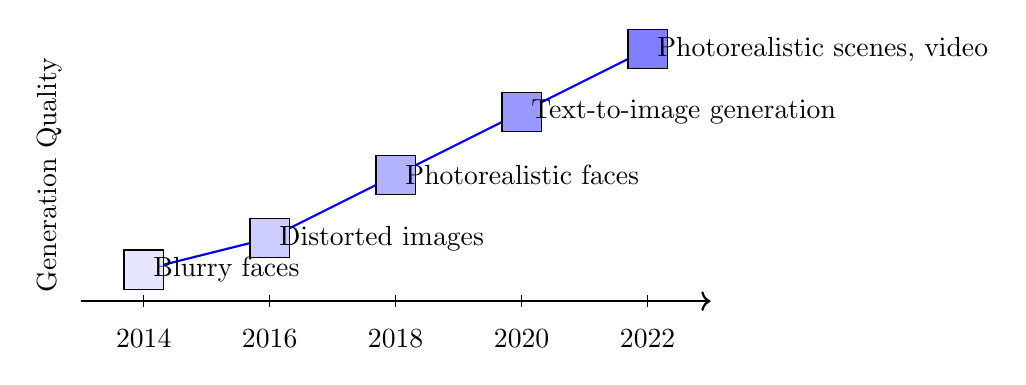
\begin{tikzpicture}[scale=0.8]
    % Draw timeline
    \draw[->, thick] (0,0) -- (10,0);
    
    % Timeline markers
    \foreach \x/\year in {1/2014, 3/2016, 5/2018, 7/2020, 9/2022} {
        \draw (\x,0.1) -- (\x,-0.1);
        \node[below] at (\x,-0.3) {\year};
    }
    
    % Quality improvement
    \draw[blue, thick] (1,0.5) -- (3,1) -- (5,2) -- (7,3) -- (9,4);
    
    % Images
    \node[draw, fill=blue!10, minimum size=0.5cm] at (1,0.5) {};
    \node[draw, fill=blue!20, minimum size=0.5cm] at (3,1) {};
    \node[draw, fill=blue!30, minimum size=0.5cm] at (5,2) {};
    \node[draw, fill=blue!40, minimum size=0.5cm] at (7,3) {};
    \node[draw, fill=blue!50, minimum size=0.5cm] at (9,4) {};
    
    % Labels
    \node[right] at (1,0.5) {Blurry faces};
    \node[right] at (3,1) {Distorted images};
    \node[right] at (5,2) {Photorealistic faces};
    \node[right] at (7,3) {Text-to-image generation};
    \node[right] at (9,4) {Photorealistic scenes, video};
    
    % Y-axis
    \node[rotate=90] at (-0.5,2) {Generation Quality};
\end{tikzpicture}
\end{center}
\end{frame}

%% Slide 26: Introduction to Autoencoders
\begin{frame}
\frametitle{Introduction to Autoencoders}
\begin{itemize}
    \item Self-supervised neural networks with two parts:
    \begin{itemize}
        \item \textbf{Encoder:} Compresses input to latent representation
        \item \textbf{Decoder:} Reconstructs input from latent representation
    \end{itemize}
    \item Training objective: Minimize reconstruction error
    \item Bridge between supervised learning and generative modeling
    \item Foundation for more advanced generative architectures
\end{itemize}
\end{frame}

%% Slide 27: Autoencoder Architecture
\begin{frame}
\frametitle{Basic Autoencoder Architecture}
\begin{center}
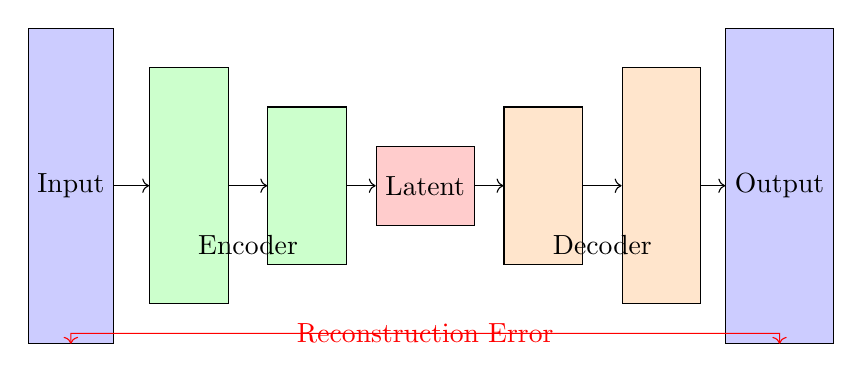
\begin{tikzpicture}[scale=0.75]
    % Input
    \node[rectangle, draw, minimum height=4cm, minimum width=1cm, fill=blue!20] (input) at (0,0) {Input};
    
    % Encoder layers
    \node[rectangle, draw, minimum height=3cm, minimum width=1cm, fill=green!20] (e1) at (2,0) {};
    \node[rectangle, draw, minimum height=2cm, minimum width=1cm, fill=green!20] (e2) at (4,0) {};
    
    % Latent representation
    \node[rectangle, draw, minimum height=1cm, minimum width=1cm, fill=red!20] (latent) at (6,0) {Latent};
    
    % Decoder layers
    \node[rectangle, draw, minimum height=2cm, minimum width=1cm, fill=orange!20] (d1) at (8,0) {};
    \node[rectangle, draw, minimum height=3cm, minimum width=1cm, fill=orange!20] (d2) at (10,0) {};
    
    % Output
    \node[rectangle, draw, minimum height=4cm, minimum width=1cm, fill=blue!20] (output) at (12,0) {Output};
    
    % Connections
    \draw[->] (input) -- (e1);
    \draw[->] (e1) -- (e2);
    \draw[->] (e2) -- (latent);
    \draw[->] (latent) -- (d1);
    \draw[->] (d1) -- (d2);
    \draw[->] (d2) -- (output);
    
    % Labels
    \node[below=0.5cm] at (3,0) {Encoder};
    \node[below=0.5cm] at (9,0) {Decoder};
    
    % Loss
    \draw[<->, red] (input) -- (0,-2.5) -- (12,-2.5) -- (output);
    \node[red] at (6,-2.5) {Reconstruction Error};
\end{tikzpicture}
\end{center}
\end{frame}

%% Slide 28: Types of Autoencoders
\begin{frame}
\frametitle{Types of Autoencoders}
\begin{itemize}
    \item \textbf{Vanilla Autoencoder:} Basic architecture
    \item \textbf{Denoising Autoencoder:} Trained to recover clean data from noisy input
    \item \textbf{Sparse Autoencoder:} Adds sparsity constraint to hidden representations
    \item \textbf{Convolutional Autoencoder:} Uses CNN architectures for images
    \item \textbf{Variational Autoencoder (VAE):} Probabilistic version with regularized latent space
\end{itemize}

\begin{center}
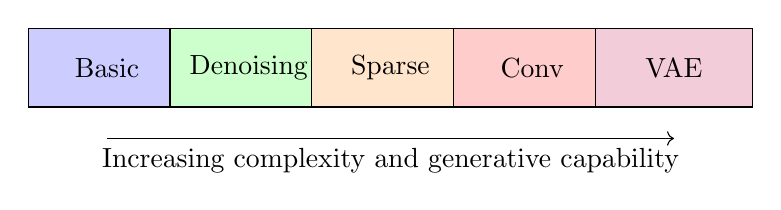
\begin{tikzpicture}[scale=0.6]
    % Autoencoder types diagram
    \node[rectangle, draw, fill=blue!20, minimum width=2cm, minimum height=1cm] (basic) at (0,0) {Basic};
    \node[rectangle, draw, fill=green!20, minimum width=2cm, minimum height=1cm] (denoising) at (3,0) {Denoising};
    \node[rectangle, draw, fill=orange!20, minimum width=2cm, minimum height=1cm] (sparse) at (6,0) {Sparse};
    \node[rectangle, draw, fill=red!20, minimum width=2cm, minimum height=1cm] (conv) at (9,0) {Conv};
    \node[rectangle, draw, fill=purple!20, minimum width=2cm, minimum height=1cm] (vae) at (12,0) {VAE};
    
    % Complexity arrow
    \draw[->] (0,-1.5) -- (12,-1.5);
    \node[below] at (6,-1.5) {Increasing complexity and generative capability};
\end{tikzpicture}
\end{center}
\end{frame}

%% Slide 29: Project Overview
\begin{frame}
\frametitle{Hands-on: Simple Autoencoder for Image Reconstruction}
\begin{itemize}
    \item Click here to download the file: \href{https://drive.google.com/file/d/1RgGwSJogVCm2UfRfpbctzQQzN3o7hRhY/view?usp=sharing}{Auto Encoder Hands On.ipynb}
\end{itemize}
\end{frame}


%% Slide 35: Connection to Advanced Generative Models
\begin{frame}
\frametitle{Connection to Advanced Generative Models}
\begin{itemize}
    \item Autoencoders establish \textbf{latent space} concept central to generative AI
    \item VAEs add probabilistic framework for generation
    \item Modern image generators (diffusion models) incorporate similar encoder-decoder structures
    \item Understanding autoencoders provides foundation for:
    \begin{itemize}
        \item GANs
        \item VAEs
        \item Diffusion Models
        \item Transformer-based generative models
    \end{itemize}
\end{itemize}
\end{frame}

%% Slide 36: Session Summary
\begin{frame}
\frametitle{Session Summary}
\begin{itemize}
    \item Explored the evolution from traditional ML to deep learning
    \item Reviewed fundamental neural network architectures
    \item Understood the transition to generative AI paradigm
    \item Implemented a simple autoencoder for image reconstruction
\end{itemize}
\end{frame}



\section{Appendix}

%%% Slide 7: Sampling Methods %%%
\begin{frame}{Sampling \& Generation}
\begin{columns}[T]
\begin{column}{0.6\textwidth}
\textbf{Key Techniques:}
\begin{itemize}
\item Ancestral Sampling
\item Markov Chain Monte Carlo (MCMC)
\item Importance Sampling
\item Rejection Sampling
\end{itemize}

\textbf{Modern Methods:}
\begin{itemize}
\item Langevin Dynamics
\item Diffusion Process
\item Normalizing Flows
\end{itemize}
\end{column}

\begin{column}{0.4\textwidth}
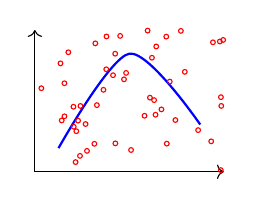
\begin{tikzpicture}[scale=0.6]
\draw[->] (0,0) -- (4,0);
\draw[->] (0,0) -- (0,3);
\draw[blue,thick] plot[smooth] coordinates {(0.5,0.5) (2,2.5) (3.5,1)};
\foreach \i in {1,...,50} {
    \draw[red] (rnd*4, rnd*3) circle (0.05);
}
\end{tikzpicture}
\end{column}
\end{columns}

\vspace{0.5cm}
\textbf{GenAI Application:} All generative models ultimately require efficient sampling from learned distributions
\end{frame}

\end{document}